%
% loesbarkeit.tex
%
% (c) 2021 Prof Dr Andreas Müller, OST Ostschweizer Fachhochscule
%
\section{Lösungen von Polynomgleichungen
\label{buch:potenzen:section:loesungen}}
\rhead{Lösungen von Polynomgleichungen}
Die Berechnung von Polynomen ist sehr einfach, da nur arithmetische 
Grundoperationen benötigt werden.
In vielen Anwendungen sind jedoch die Argumente gefragt, für die ein
Polynom einen bestimmten Wert annimmt.
Es geht also um die Lösung von Gleichungen der Form
\[
p(x) = c
\]
für ein Polynome $p(x)$ und eine Konstante $c\in\mathbb{C}$.

%
% Fundamentalsatz der Algebra
%
\subsection{Fundamentalsatz der Algebra}
In Abschnitt~\ref{buch:polynome:subsection:faktorisierung-und-nullstellen}
wurde gezeigt, dass sich jede Nullstellen $\alpha$ eines Polynoms als
Faktor $x-\alpha$ abspalten lässt.
Jedes Polynom liess sich in ein Produkt von Linearfaktoren und
einen Faktor zerlegen, der keine Nullstellen hat.
Zum Beispiel hat das Polynom $x^2+1\in\mathbb{R}[x]$ keine
Nullstellen in $\mathbb{R}$.
Eine solche Nullstelle müsste eine Quadratwurzel von $-1$ sein.
Die komplexen Zahlen $\mathbb{C}$ wurden genau mit dem Ziel konstruiert,
dass $i=\sqrt{-1}$ sinnvoll wird.
Der Fundamentalsatz der Algebra zeigt, dass $\mathbb{C}$ alle
Nullstellen von Polynomen enthält.

\begin{satz}[Gauss]
\index{Satz!Fundamentalsatz der Algebra}%
\index{Fundamentalsatz der Algebra}%
\label{buch:potenzen:satz:fundamentalsatz}
Jedes Polynom $p(x)=a_nx^n+\dots + a_2x^2 + a_1x + a_0\in\mathbb{C}[x]$
zerfällt in ein Produkt
\[
p(x)
=
a_n
(x-\alpha_1)(x-\alpha_2)\cdots(x-\alpha_n)
\]
für Nullstellen $\alpha_k\in\mathbb{C}$.
\end{satz}


%
% Lösbarkeit durch Wurzelausdrücke
%
\subsection{Lösbarkeit durch Wurzelausdrücke}
Der Fundamentalsatz macht keine Aussage darüber, wie die Nullstellen
eines Polynoms gefunden werden können.
Selbst für besonders einfache Gleichungen der Form
\[
x^n = c
\qquad
\text{oder Polynome der Form}
\qquad
p(x) = x^n -c
\]
gibt es keine direkte, nur auf den arithmetischen
Operationen basierende Methode, eine Nullstelle oder Faktorisierung
in endlich vielen Schritten zu finden.
Dies rechtfertigt, für diese einfachen Fälle eine neue, spezielle
Funktion zu definieren, die mindestens für reelle Koeffizienten 
die Nullstelle als Rückgabewert hat.

\begin{figure}
\centering
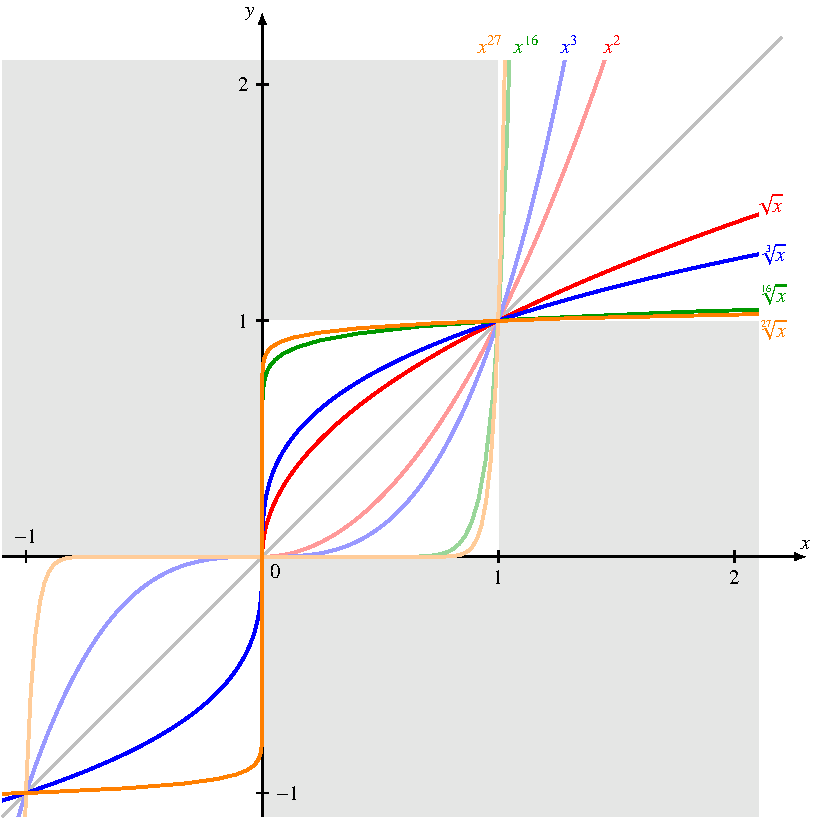
\includegraphics{chapters/010-potenzen/images/wurzel.pdf}
\caption[Graph der Wurzelfunktionen]{Graph der Wurzelfunktionen
\ensuremath{x\mapsto\root{n}\of{x}}
als Umkehrfunktionen der Potenzfunktionen $x\mapsto x^n$ für
$n=2$ ({\color{red}rot}), $n=3$ ({\color{blue}blau}),
$n=16$ ({\color{darkgreen}grün}) und $n=27$ ({\color{orange}orange}).
\label{buch:potenzen:fig:wurzel}
}
\end{figure}

\begin{definition}
Die inverse Funktion der Potenzfunktion
$f\colon \mathbb{R}\to\mathbb{R}:x\mapsto y=f(x)=x^n$
heisst die $n$-{\em te Wurzel} und wird
\[
\root{n}\of{\mathstrut\phantom{m}}
=
f^{-1}
\colon
D\to\mathbb{R}
:
y\mapsto f^{-1}(y)=\root{n}\of{\mathstrut y}
\]
geschrieben.
Für gerades $n$ ist der Definitionsbereich der Wurzel nur
$D=\mathbb{R}_{\ge 0}$, für ungerades $n$ ist $D=\mathbb{R}$.
Für $n=2$ wird die Wurzel als
\(
\root{2}\of{\mathstrut y}
=
\sqrt{\mathstrut y}
\)
geschrieben.
\end{definition}

Mit der Wurzelfunktion ist es jetzt möglich, auch kompliziertere
Gleichungen zu lösen:
\begin{enumerate}
\item
Für negative Argument $y<0$ müssen Quadratwurzeln als
$\sqrt{y\mathstrut}=i\sqrt{-y\mathstrut}$ definiert werden.
\item
Mindestens der Betrag der Wurzel einer komplexen Zahl lässt
sich jetzt sofort mittels $|\root{n}\of{c\mathstrut}|=\root{n}\of{|c|\mathstrut}$
berechnen.
Für das Argument sind jedoch die in
Abschnitt~\label{buch:geometrie:section:trigonometrisch} definierten
trigonometrischen Funktionen notwendig.
\item
Die quadratische Gleichung 
\[
ax^2+bx+c=0
\]
hat die Nullstellen
\[
x_{1,2} = \frac{-b\pm\sqrt{b^2-4ac\mathstrut}}{2a}.
\]
\item
Für kubische Gleichungen hat Cardano eine Lösung gefunden, die
Nur Wurzelausdrücke und arithmetische Operationen verwendet.
Die Gleichung $x^3+px+q=0$ hat die Nullstelle
\[
x
=
\root{3}\of{-\frac{q}2+\sqrt{\frac{q^2}4+\frac{p^3}{27}}}
+
\root{3}\of{-\frac{q}2-\sqrt{\frac{q^2}4+\frac{p^3}{27}}}.
\]
Falls das Argument der Quadratwurzel negativ ist, muss eine
Kubikwurzel aus einer komplexen Zahl berechnet werden, was
wieder über die Möglichkeiten der oben definierten Wurzelfunktionen
hinausgeht.
\item
Für die Lösung einer Gleichung vierten Grades hat Ferrari eine
Formel angegeben, die mit Wurzelausdrücken und arithmetischen
Operationen auskommt.
\end{enumerate}

Allerdings ist damit auch bereits ausgeschöpft, was die
Wurzelfunktionen zur Lösung von Polynomgleichungen beitragen
können.
Der folgende Satz von Abel zeigt, dass man für Polynomgleichungen
höheren Grades nicht mit einer Lösung durch Wurzelausdrücke
rechnen kann.

\begin{satz}[Abel]
\index{Satz!von Abel}
\label{buch:potenzen:satz:abel}
Für Polynomegleichungen vom Grad $n\ge 5$ gibt es keine allgemeine
Lösung durch Wurzelausdrücke.
\end{satz}



%
% Algebraische Zahlen
%
\subsection{Algebraische Zahlen}
Die Verwendung der komplexen Zahlen ist für numerische Rechnungen
zweckmässig.
In den Anwendungen der Computer-Algebra hingegen erwartet man zum
Beispiel exakte Formeln für eine Stammfunktion.
Nicht rationale Zahlen können nur exakt verarbeitet werden, wenn
Sie sich algebraisch in endlich vielen Schritten charakterisieren
lassen.
Dies ist zum Beispiel für rationale Zahlen $\mathbb{Q}$ möglich.
Gewisse irrationale Zahlen kann man charakterisieren durch 
die Eigenschaft, Nullstelle eines Polynoms $p(x)\in\mathbb{Q}[x]$
mit rationalen Koeffizienten zu sein.

\begin{definition}
Eine Zahl $\alpha$ heisst {\em algebraisch} über $\mathbb{Q}$,
wenn es ein Polynom
\index{algebraische Zahl}%
$p(x)\in \mathbb{Q}[x]$ gibt, welches $\alpha$ als Nullstelle hat.
Eine Zahl heisst transzendent über $\mathbb{Q}$, wenn sie nicht algebraisch ist
über $\mathbb{Q}$.
\end{definition}

Die Zahlen $i=\sqrt{-1}$ und $\sqrt{n\mathstrut}$ für $n\in\mathbb{N}$
sind also algebraisch über $\mathbb{Z}$.
Es ist gezeigt worden, dass $\pi$ und $e$ nicht nur irrational
sind, sondern sogar transzendent.

Eine Polynomgleichung $p(\alpha)=0$ mit $p(x)\in\mathbb{Q}[x]$
hat eine Rechenregel für $\alpha$ zur Folge.
Dazu schreibt man
\[
p_n\alpha^n + p_{n-1}\alpha^{n-1} + \dots + a_1\alpha + a_0 =0
\qquad\Rightarrow\qquad
\alpha^n = -\frac{1}{p_n}\bigl(
p_{n-1}\alpha^{n-1}+\dots+a_1\alpha+a_0
\bigr).
\]
Diese Regel erlaubt, jede Potenz $\alpha^k$ mit $k\ge n$ durch
Potenzen von $\alpha^l$ mit $l<n$ auszudrücken.
Die Zahlen, die sich durch arithmetische Operationen aus
$\alpha$ bilden lassen, lassen sich also sogar durch lineare
Operationen aus $1,\alpha,\alpha^2,\dots,\alpha^{n-1}$
bilden.
Sie bilden einen endlichdimensionalen Vektorraum über $\mathbb{Q}$.
Rechnen mit algebraischen Zahlen ist also in einem CAS exakt möglich,
wie das in Abschnitt~\ref{buch:integrale:section:dkoerper}
für die Berechnung von Stammfunktionen illustriert wird.


